\chapter{Longlist verschillende AR / VR technologieën}
\label{ch:longlist}

Hierin worden de verschillende technologieën overlopen die kunnen gebruikt worden om deze use case te volbrengen.
Bij elke technologie zal er dan worden gezegd waarom deze voldoet of niet voldoet aan de eisen (TODO) van de use case.

\section{Head Mounted Virtual Reality}
Bij head mounted virtual reality wordt er gebruik gemaakt van een HDM (head-mounted-display) die de gebruiker op zijn hoofd zet. Deze headset zal dan een virtuele wereld tonen die volledig aangestuurd is door de applicatie zelf. Deze wereld zal dus geen rekening houden met de echte wereld, dit kan hierdoor wel voor problemen zorgen indien er geen sensor of camera aanwezig is die je tegenhoud om tegen muren te lopen.

HMD kan over 3DOF of 6DOF beschikken afhankelijk van de gebruikte headset. De 3DOF headsets zijn wel goedkoper dan de 6DOF en maken vaak gebruik van de smartphone om zo het beeld te kunnen tonen. 
% TODO CONTENT Iets over het beeld dat in 2 wordt gesplitst, op elke oog 1 beeld
% TODO ASK Is uitleg over hoe het beeld op de ogen wordt geprojecteerd en geinterpreteerd door de hersenen teveel of topic?
\subsection{Medische Klachten}
Sommige mensen kunnen bij het gebruik van een HDM ziek of misselijk worden. Dit wordt meestal veroorzaakt door een te klein of onnatuurlijk gezichtsveld (Field-Of-View, FoV) (INSERT CITE) of als de beweging in de applicatie wordt gedaan a.h.v. teleportatie. (INSERT CITE) Deze teleportatie beweging komt vooral voor bij 3DOF omdat hierbij er manieren zijn om de camerea te bewegen, namelijk teleportatie of via een joystick.

De tijd tussen de beweging in de echte wereld en de virtuele kan ook invloed hebben op virtual reality sickness indien deze te hoog is \autocite{Elbamby2018} en \autocite{DiZio2000}. 
% TODO TRANSLATE disconnection
Veel van deze problemen hebben te maken met de staat van de huidige hardware en hoe deze geen hogere FoV aan een hoge framerate kunnen ondersteunen. Een hoge en stabiele framerate is nodig indien om de gebruiker een aangename ervaring te geven. Een te lage framerate kan ervoor zorgen dat er (TRANSLATE) disconnection is tussen de beweging van de gebruiker en het gene dat effectief op het scherm gebeurt, dit kan voor frustratie zorgen.
\subsection{Sensoren}
% TODO ASK Extra uitleg over IMU of niet?
De soorten sensoren die gebruikt worden bij een HMD hangt af van de gewenste bewegingen. Als er alleen maar rotationale bewegingen nodig zijn kan een gyroscoop of een IMU, inertial measurement unit (bij standalone headsets) worden gebruikt om zo de yaw, pitch, roll te kunnen meten en hierop te kunnen reageren \autocite{LaValle2014}. Indien er ook positionale bewegingen nodig zijn moeten er infraroodsensoren in de kamer worden geplaatst om zo de headset te kunnen tracken. Deze sensoren zorgen er wel voor dat er meer voorbereiding nodig is alvorens de headset kan worden gebruikt.
\subsection{Realisme}
Omdat de headset het beeld op de beide ogen projecteert is er geen besef van de echte wereld en kan de virtuele wereld makkelijker als 'echt' worden ervaart. De headset zal ook gemonteerd zijn op het hoofd waardoor beide handen vrij zijn om acties uit te voeren. Hierdoor kunnen beide handen ook worden gezien in de virtuele wereld wat de ervaring nog meer realistischer maakt.
% TODO CONTENT Iets over latency => tijd tussen beweging hoofd en beweging in vr
\subsection{Interactiviteit}
De manier waarop de gebruiker zal interageren met de virtuele wereld zal afhangen van het aantal vrijheidsgraden bij 6DOF zal hij de mogelijkheid hebben om zelf te kunnen rondlopen in de wereld terwijl bij 3DOF dit a.h.v. een joystick of via teleportatie zal moeten. Er is ook altijd de mogelijkheid om controllers te gebruiken. Deze controllers zullen dan de mogelijkheid bieden om fysieke interacties te kunnen doen, bijvoorbeeld het oppakken van een virtueel object of door op één van de knoppen van de controller te duwen een actie uit te voeren.

\begin{figure}
    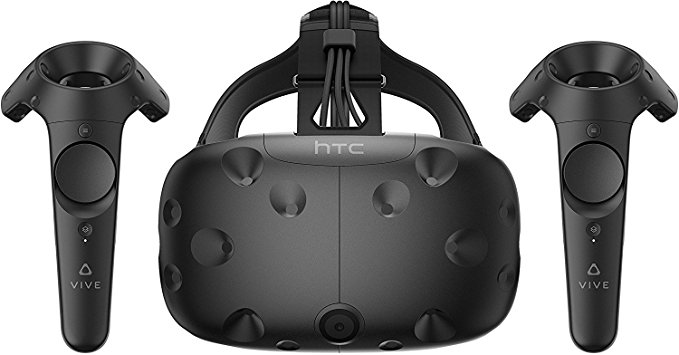
\includegraphics[width=\linewidth]{headset.jpg}
    \caption{HTC Vive headset en controllers}
    \label{fig:htcvive}
\end{figure}

\subsection{Bruikbaarheid}
De bruikbaarheid van HMD in musea is nogal laag. Het is niet echt praktisch om gebruikers met een HMD (Google Cardboard of Full HMD) te laten rondlopen omdat dit veel ruimte in het museum zou kosten om goed te implementeren. Indien er toch zou worden gekozen om dit te implementeren kan bij er ook een hoge financiele kost aanhangen. Afhankelijk of de gebruikers moeten langskomen voor de applicatie uit te proberen of niet kan het zijn dat het museum headsets moet aankopen en hiervoor een speciale ruimte moet inrichten.

Meeste mensen die naar een museum gaan willen juist rondlopen in het museum zelf rondlopen en niet in de virtuele versie hiervan. Het is daarom ook niet echt logisch om een HMD hiervoor te gebruiken. Natuurlijk als het museum wil gaan voor een ervaring zoals bij het Historium Brugge kan HMD wel op een goede manier worden gebruikt.

\section{Augmented Reality} \label{sec:augmentedreality}
Augmented reality kan het best worden omschreven als het plaatsen van virtuele objecten in de echte wereld maar zonder de mogelijkheid om fysiek te reageren met deze objecten. Meestal wordt er voor deze technologie geen headset gebruikt maar eerder gewoon een smartphone. Er bestaan wel verschillende headsets voor augmented reality waar de smartphone in geplaatst kan worden \autocite{Schops2014}.

\subsection{Plane Detection}
Om virtuele objecten in de echte wereld te kunnen plaatsen moet de echte wereld eerst gemapped. Dit gebeurt a.h.v. computer vision om zo te weten waar een nieuwe plane begint en eindigt. Dit algoritme zal constant lopen om zo nieuwe planes te kunnen ontdekken \autocite{Xu2018}. Het algoritme dat hiervoor wordt gebruikt zal een vorm zijn van odometry tracking.

Eens een plane ontdekt is kan deze worden gebruikt om nieuwe objecten op te plaatsen. De applicatie zal dan het object verbinden aan een ankerpunt (INSERT CITE). Door dit ankerpunt kan de locatie van het object worden onthouden zelfs als de gebruiker wat verder weg wandelend. Er zijn echter wel limieten aan dit anker, indien de gebruiker te ver weg gaat van het punt en nadien terug komt zal het virtuele object verplaatst zijn, dit begrip noemt drifting \autocite{You1999}. Indien er grote precisie nodig is voor de applicatie kan dit wel problemen zorgen.

\subsection{Odometry Tracking}

Door gebruik te maken van de IMU en dus ook de gyroscope en accelerometers die in een smartphone zitten heeft deze de mogelijkheid om vlakken te herkennen maar ook om zo achteraf terug te kunnen weten welke gebieden er al gescand zijn geweest. \autocite{Leutenegger2015}

De twee grote native AR frameworks maken hier beide gebruik van. De techniek die ARCore gebruikt noemt 'concurrent odometry and mapping' (INSERT CITE GOOGLE) terwijl de gebruikte techniek van ARKit 'visual-inertial odometry' (INSERT CITE APPLE) noemt. 

Beide technieken werken echter wel op dezelfde manier. Het algoritme combineert de motion data van de smartphone met de herkende features van het camerabeeld en berekent zo de verandering in positie. Hierdoor kunnen de juiste anchors en dus hun objecten worden getoond (INSERT CITE APPLE) (INSERT CITE GOOGLE).

Omdat er rekening wordt gehouden met het camerabeeld hangt de accuraatheid van het algoritme af van dit beeld. Als er bijvoorbeeld te weinig licht is zal het algoritme de locatie niet kunnen herkennen. (INSERT CITE APPLE).

\begin{figure}
    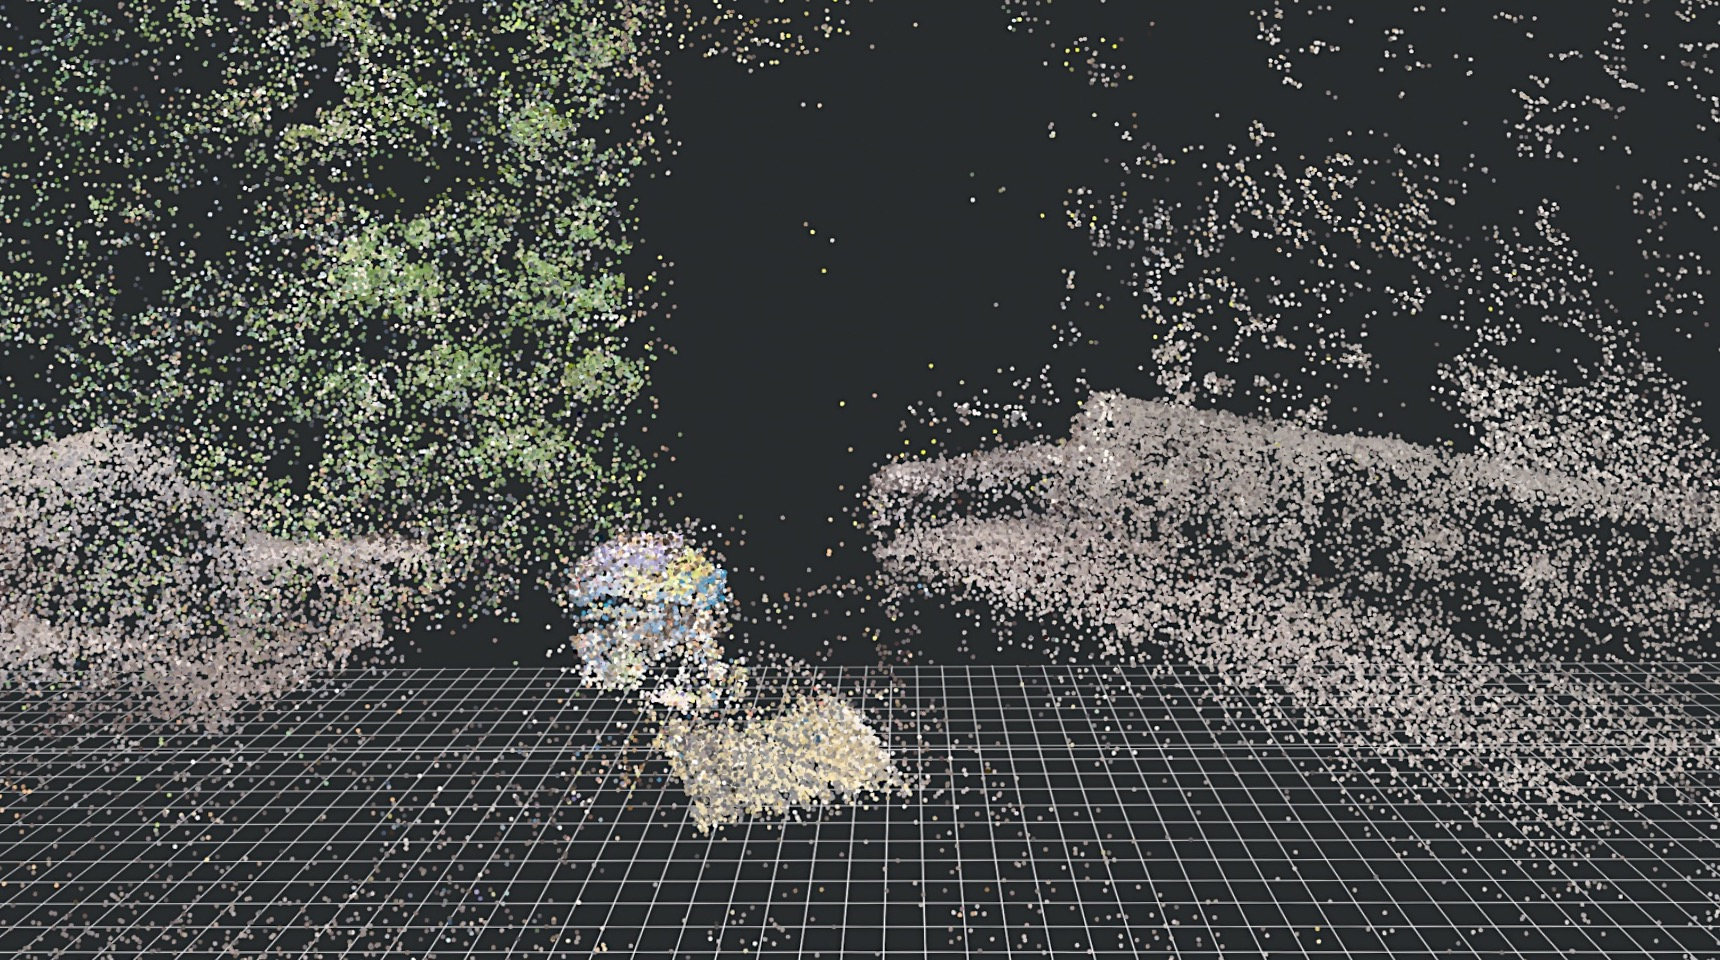
\includegraphics[width=\linewidth]{pointcloudarkit.jpg}
    \caption{ARKit Visual-Inertial Odometry}
    \label{fig:pointcloudarkit}
\end{figure}


% TODO IMAGE Point cloud / plane detection
% TODO CITE Object Anchor, alleen maar concrete implementaties gevonden ARCORE / ARKIT https://developers.google.com/ar/develop/developer-guides/anchors
\subsection{Image Recognition}
Een tweede manier om virtuele objecten in de wereld te plaatsen is met image recognition. Ook hierbij wordt gebruik gemaakt van computer vision zoals te zien op figuur \ref{fig:imagereg}.

Hierbij zal de image worden gebruikt als ankerpunt om de virtuele objecten op te plaatsen en te onthouden. Eens de image herkent is kunnen de objecten erop worden geplaatst. Wanneer de smartphone de afbeelding niet meer kan zien zal deze de positie van het object, na een tijdje, vergeten en zal tracking worden uitgezet. Vanaf de smartphone de afbeelding weer herkent kan het terug worden weergegeven.

Een alternatief van image recognition is object recognition. In plaats van een 2d afbeelding wordt er hier een 3d object gebruikt dat wordt herkent (INSERT CITE VUFORIA).

\begin{figure}
    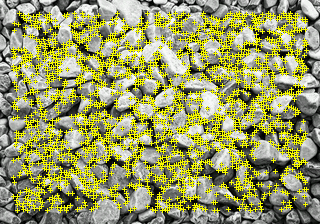
\includegraphics[width=\linewidth]{vuforiaImageReg.png}
    \caption{Aangeduide features op een afbeelding}
    \label{fig:imagereg}
\end{figure}

\subsection{Realisme}
Omdat augmented reality geen besef heeft van aanpassingen in de wereld, bv een persoon die voor de camera loopt is het soms wel moeilijk om een immersieve ervaring te maken. Dit is vooral omdat de huidige hardware van een smartphone het niet aankan om constant op zoek te gaan naar kleine veranderingen terwijl een HoloLens (Mixed Reality) dit bijvoorbeeld wel kan.

Er zijn wel nog extra technieken die frameworks kunnen gebruiken om toch nog wat extra immersie te creëren zoals light estimation. Bij dit kunnen virtuele objecten reageren wanneer de echte wereld lichter of donkerder wordt (INSERT CITE GOOGLE).

\subsection{Interactiviteit}
Het gebruik van een smartphone kan de interactiviteit van een applicatie verminderen omdat de gebruiker deze moet vasthouden en dus maar één hand vrij heeft. Dit probleem kan echter wel worden opgelost indien er een augmented reality headset wordt gebruikt.

De virtuele wereld zal wel nooit echt reageren op fysieke handelingen wat er dus voor zorgt dat elke actie op het scherm van de smartphone moet gebeuren.

Alhoewel deze twee zaken als grote nadelen kunnen gezien worden kan men hier ook gebruik van maken. Aangezien de smartphone in de hand is kunnen ook niet augmented reality zaken worden gebruikt. Er kan bijvoorbeeld een menu zijn waar de gebruiker verschillende rondleidingen uit kan kiezen.

\subsection{Bruikbaarheid}
Het gebrek aan een kabel bij augmented reality zorgt er voor dat dit op vele plaatsen kan gebruikt worden. Vooral bij musea is dit handig omdat het hele museum kan gebruikt worden en er geen speciale ruimtes nodig zijn.

Vele mensen die naar musea gaan hebben vaak hun smartphone bij wat er dus voor zorgt dat de gebruiker alleen een app nodig heeft om mee te doen aan de ervaring.

Image en object recognition is ook iets dat heel makkelijk kan gebruikt worden in musea omdat bestaande kunstwerken kunnen dienen als objecten waar de virtuele content op kan worden getoond.

\section{360 Degrees Videos}
360 Degrees Videos is de simpelste vorm van virtual reality in deze longlist. Eigenlijk zijn dit gewoon videos waarbij de gebruiker de camera 360 graden kan draaien \autocite{Hosseini2016}.

Om deze video's te bekijken is er eigenlijk niets speciaal nodig. Als een 360 graden video op een desktop wordt bekeken zal de camera nog altijd kunnen draaien door middel van de pijltjestoetsen. Terwijl wanneer deze op een apparaat met een IMU zal draaien door met het apparaat te bewegen. Wanneer er een IMU wordt gebruikt kan er nog altijd een onderscheid tussen een HMD en een gewoon apparaat. Als een HMD aanwezig zal de video worden getoond in VR. Bij een gewoon device zal de video echter zoals een normale video worden getoond maar wel met de mogelijkheid om de camera te draaien.

\subsection{Recording}
Het opnemen van deze video is wel iets ingewikkelder. Er zijn twee formaten om een 360 graden video voor te stellen namelijk equirectangular en cubic \autocite{Lee2010}. 

Bij het equirectangular formaat wordt elke frame van de video op een vlakke afbeelding geprojecteerd. Deze afbeelding kan dan op een bol worden gelegd en deze bol zal de video voorstellen. Een makkelijke manier om een equirectangular afbeelding voor te stellen is namelijk een wereldkaart. Wanneer men een wereldkaart op een bol legt zal deze een wereldbol worden.
 
\begin{figure}
    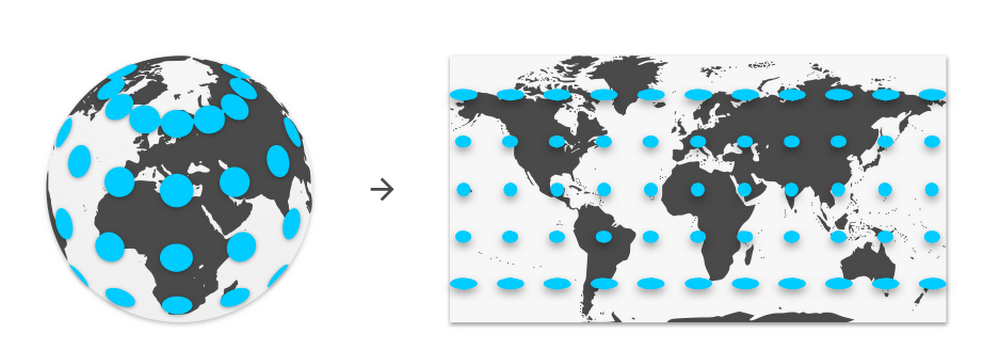
\includegraphics[width=\linewidth]{equirectangular.png}
    \caption{Een equirectangular projectie van de wereld}
    \label{fig:equirectangularprojection}
\end{figure}

Het cubic formaat werkt ongeveer op dezelfde manier behalve dat hierbij de frame zal worden opgedeeld in zes afbeeldingen die elk een zijde van de kubus zal voorstellen.

% TODO ASK Uitleg van projectie op vlakke afbeelding?
\subsection{Realisme}
Een 360 graden video kan bestaan uit echte beelden of virtuele beelden op die manier zijn er veel mogelijkheden om deze video immersief te maken. 

Wanneer men kijkt naar de sensorama kan men zien dat dit eigenlijk ook een 360 graden video is. Hier werd de ervaring immersief gemaakt door de zintuigen te stimuleren en zoals al eerder vermeld is dit één van de belangrijkste manieren waarop het gevoel van realisme kan worden opgewekt.

\subsection{Interactiviteit}
Het enigste wat een gebruiker kan doen bij een 360 graden video is het ronddraaien van de camera hierdoor is de interactiviteit minimaal. Toch zijn er 360 apps die net iets meer interactiviteit hebben, bij deze is er bijvoorbeeld de mogelijkheid om naar objecten te kijken en daarover informatie te tonen. Of er kunnen voorwerpen in de video worden verstopt die de gebruiker moet vinden. 
\subsection{Bruikbaarheid}
Omdat de video op elk apparaat dat Youtube of een andere 360 player ondersteund kan draaien is het heel bruikbaar. Echter om de volledige ervaring te krijgen wordt er best wel gebruik gemaakt van een HMD.

Hierbij komt echter hetzelfde probleem voor als bij virtual reality. Het is niet echt logisch dat dit wordt gebruikt in musea want gebruikers komen naar het museum om het fysiek te bezoeken en niet virtueel.

\section{Mixed Reality} \label{sec:mixedreality}
Ook hierbij wordt er gebruik gemaakt van een HDM. Het grote verschil met virtual reality is dat er bij mixed reality ook rekening wordt gehouden met de echte wereld. Een mixed reality headset heeft namelijk de mogelijkheid om de echte wereld te mappen naar een virtuele wereld a.h.v. de camera die langs de voorkant gemonteerd is.

Een mixed reality headset is ook uitgerust met verschillende sensoren om de positie binnen in de wereld te volgen. Door de combinatie van de mapping en sensoren is het dus niet nodig om extra sensoren te plaatsen om room-scale VR te te gebruiken.
\subsection{Spatial Mapping}
Het algoritme dat gebruikt wordt voor de mapping is spatial mapping. Dit algoritme % TODO CONTENT Uitleg spatial mapping
\subsection{Realisme}
\subsection{Interactiviteit}
\subsection{Bruikbaarheid}
% TODO ASK Uitleg gyropscoop? te ingewikkeld?
% TODO CONTENT Depth Camera
% TODO CONTENT Alternative devices? AR glasses? Future of?